\chapter{Validation}

  This chapter will go through all the validation and tests implemented to measure the perfomance and the correct functioning of the new behaviors. 

  To validate each implemented behavior we propose using them both in simulation and in real flight missions. The validation tests are presented in detail in section \ref{ch_5:sect:val_tests}, explaining what the tests measure and how they do it as well as the intuition behind each test. Afterwards, in section \ref{ch_5:subsect:exp_simulation} we will epose the simulator used and it's particularities as well as how it is integrated with the current version of Aerostack. It will be followed by the specification of the aircraft used for the real flight mission in section \ref{ch_5:sect:real_flight} to finish with some conclusions in section \ref{ch_5:sect:conclusions}.

\section{Validation Tests} \label{ch_5:sect:val_tests}

  A validation test should ensure that the behavior complies with the following constraints:

  \begin{enumerate}
    \item \underline{Functioning}: It should do what it is supposed to do. No more, no less.
    % \item \underline{Predictability}: All uses cases must be contemplated. No unknown states should be possible.
    \item \underline{Compatibility}: It should be compatible with the Aerostack framework architecture.
    \item \underline{Independency}: It should work independently of the UAV in use.
  \end{enumerate}

  The first constraint is the most obvious, a behavior is designed to do a concrete task. It should do only what is designed to do. The idea behind a behavior is to encapsulate a concrete algorithm, it can be the layer that encapsulates the algorithm, providing a standard API access, but it can only be one functionality.

  To test this constraint we will provide both a simulation and a real mission and put to work each behavior independently, testing that each one works as expected.

  % Predictability is always a desirable property in software development, but very tricky to ensure, that is the reason why, in software business, there is always a team decicated solely to test the software, many criterias can be applied here. In our case, we will test the predictability of the behavior functionality, not the software itself. This means that we will test that, for each behavior, all case studies are covered: the correct sensors are available, the algorithm process is effectively running, the behavior knows how to interpret the output of the algorithm it monitors, etc. More specifically, we will test this cases to grasp an intuition about what to do when those criterias fail. The real world is full of randomness and uncertainty and hardware is usually not realiable enough, these reasons place this constraint as the hardest to test.

  Ensuring a peace of software is compatible with another one is much easier than covering all possible uses cases in an unpredictable environment, furthermore, as we expect all the data accessed by a behavior to be in a certain format (and ensured through static, c++ compilation), this constraint should be straightforward. Nevertheless, there are some considerations to be taken care of here. To follow the Aerostack architecture, a behavior should always inherit the behavior class, implementing the functions imposed by it. Also, when getting data from the outside (from the rest of Aerostack, standard), extreme values should be tested, for example, sending an infite double or \textit{nan} value to a controller can effectively be a problem.

  The last constraint comes from the idea that behaviors depend upon the available features, independently of the data, if a drone has a lidar sensor, the behavior that does licalization based on lidar should work on any lidar, independently of the brand of the sensor and the drone featuring it. To ensure this constraint software based abstraction layers should be placed to handle the sensors and it's data format, providing uniform APIs, this is the case of the path planner module implemented in the Navigation interface, that abstracts the real planner so that any behavior can access it in a unified format, independently of the underlying planner.

\pagebreak

\section{Simulation} \label{ch_5:sect:simulation}

  The chosen simulator for these tests is \href{http://gazebosim.org/}{Gazebo Sim}, an open source, multiplatform, robot simulator. It was chosen because of it's open source nature, ease of use and great integration with ROS. Gazebo features an open modular, plugin based architecture, which makes it perfect to integrate new components and open the door for modules being simulated inside it and the outside world. In our case, to communicate the simulated UAV with ROS and the Aerostack framework.

  In order to convey the simulator with ROS we will employ an already made plugin called \href{https://github.com/ethz-asl/rotors_simulator/wiki}{RotorS} \cite{rotors2016}. RotorS provides some UAV models and a plugin that translates gazebo topics to ROS ones, unifying the access to the data. This architecture is perfect for any robotic environment as it minimizes the overhead of changing from simulation to real flight, as long as the topics are called the same, the Aerostack framework does not even notice it.

  As all the simulation is launched with configuration files and was done with flexibility in mind, we could adapt the already available configurations to our needs, minimizing the overhead of naming topics to our conventions.

  To choose a UAV model from the available ones we looked up for one that matches our requirements, namely a lidar sensor (hokuyo if possible), a front camera and an altitude sensor. RotorS provides a UAV modeled after the \href{http://www.asctec.de/en/uav-uas-drones-rpas-roav/asctec-hummingbird/}{AscTec Hummingbird} drone, which meets all our requirements.

  \textbf{[ToDo := Add picture of the simulator??]}

\section{Real Flight} \label{ch_5:sect:real_flight}

  Our requirements came mainly because of the implemented behaviors, which in turn came from the available hardware in the research group. Currently, the aircraft used for the most important missions is a \href{https://www.dji.com/es/matrice100}{Matrice 100} from DJI with all the sensorization cited above.

  This is used because of it's extendability (any sensor platform can be plugged in), open API and powerful motors. It's verstaile enough to provide a testbed for many research experiments and the battery lasts enough for medium duration missions.

  \textbf{[ToDo := Add picture of the drone??]}

\section{Testing Mission} \label{ch_5:sect:testing_mission}

  To provide the most realistic environment possible, the mission used to conduct all the experiments will be based in a real assignment requested to the research group a few months ago. The mission consists in inspecting the internal facade of a plant's boiler. At the time of request this new navigation interface was not implemented, so the flight was made almost by hand. In fact, this inteface was proposed after the need of an autonomous flight navigator whith the available hardware.

  The idea behind the mission is to fly a drone along the facade filming all the breathers, after the mission is completed, the film is extracted and given to the plant experts for their analysis. Additionally, a handmade mission could be very costly for the gas company as they would have had to install a portable crane and put a human to do the inspection of the 40 meters long facade.

  A human commanded drone accomplished the whole inspection in about thirty minutes. Furthermore, even in that case it was challenging for the human operator as he had to fly near the wall, which causes the drone to destabilize due to the air flows. This is the point where autonomous navigation comes in. In an autonomous mission, the control loop can be closed with any parameter that can be measured, in this case, the go to point behavior could have been employed to make the aircraft fly upwards until the whole boiler is inspected and then commanded back to land at a certain point.

  As the job is already done it is not possible to replicate it, we propose to simulate a boiler in Gazebo that resembles to real mission and the inspection of an internal facade in a building for the real flight.

  The next sections will deepen in all details of the conduted experiments and the results obtained during the tests.

\section{Experiments} \label{ch_5:sect:experiments}

  As mentioned before, for each behavior we will ensure it complies with our constraints: correct functioning, compatibility and independency. 
  % predictability , 
  
  Compatibility and independency are tested by putting the system to work, if all the code compiles and can be started, the next step is to activate each behavior through the behavior coordinator.

  Once the whole Aerostack system is deployed, the first test for each behavior consists in checking it's activation conditions, i.e.: the \textit{behavior self localize and map by lidar} cannot work without a lidar, deploying the whole Aerostack in a lidar-less UAV should cause the behavior to be deactivated instantly.

  This way we tested all conditions and capabilities of all the proposed behaviors. As this is all software related, we easily corrected all the bugs found. One example of this was the access to the path planner module: The new planner (\textit{move base}) can only plan to one goal, this makes all the behaviors requiring this module mutually incompatible, namely, the behavior that generates paths cannot work simultaneously with that of the go to point . In the same fashion the behaviors that make use of the trajectory planner cannot work together or a collision could occur.

  For the functioning constraint we setup both the real and simulated missions with a python script that commands the Aerostack, if after doing a certain amount of missions, the behaviors work as expected we consider that they work correctly. 
  
  % Predictability was trickier to check, in this case we only tested it in simulation as it could be potentially dangerous to do it with the real aircraft. During the execution of the missions we disconected the lidar sensor to check

  The following subsections explain the implemented mission for each behavior. Note that, the first two missions where only tested on the simulated environment to minimize the human operator time needed for the tests. For all missions both the simulation and the real environments used are the same, nothing was changed in the environment.

  \subsection{Behavior Generate Path in Occupancy Grid} \label{ch_5:subsect:behav_genpath_mission}

    This mission was only tested in simulation, it consisted in generating a path for every point in the go to point mission (sect. \ref{ch_5:subsect:behav_gtp_mission}). After the mission is finished, $6$ paths should be present in the belief memmory. Therefore the mission can be described as follows:
    
    \begin{enumerate}
      \item Generate path for point: ([0, 0, 1.5])
      \item Generate path for point: ([1, 0, 1.5])
      \item Generate path for point: ([1, 0, 10])
      \item Generate path for point: ([1, -5, 10])
      \item Generate path for point: ([0, -5, 1.5])
      \item Generate path for point: ([0, -5, 1])
    \end{enumerate}

    At the end of the mission we will save all the generated paths to used them as the input for the next behavior's mission.

  \subsection{Behavior Follow Path in Occupancy Grid} \label{ch_5:subsect:behav_fpath_mission}

    In this mission we took all the generated paths and tested the execution one by one. It's worth noting that as each path was generated from the inital point, we will interleave the execution of each path with a reset, as the drone has to start on the [0, 0] coordinate always. In this way, the mission generated is:

    \begin{enumerate}
      \item Follow path for point: ([0, 0, 1.5])
      \item Follow path for point: ([1, 0, 1.5])
      \item Follow path for point: ([1, 0, 10])
      \item Follow path for point: ([1, -5, 10])
      \item Follow path for point: ([0, -5, 1.5])
      \item Follow path for point: ([0, -5, 1])
    \end{enumerate}

  \subsection{Behavior Go To Point in Occupancy Grid} \label{ch_5:subsect:behav_gtp_mission}

    \begin{enumerate}
      \item Take Off
      \item Go to $1.5$ meters height ([0, 0, 1.5])
      \item Go to $1$ meter to the front, maintaining the altitude. ([1, 0, 1.5])
      \item Go to $10$ meters height, maintaining the same distance to the wall. ([1, 0, 10])
      \item Go to $5$ meters to the right, keeping the same distance and altitude. ([1, -5, 10])
      \item Go to $1$ meter away from the wall, maintaining the same altitude. ([0, -5, 1.5])
      \item Go to $1$ meter height, maintaining the same distance to the wall. ([0, -5, 1])
      \item Land
    \end{enumerate}

    This a similar mission to the one carried out in the boiler. All the python code for this mission can be found in the appendix \ref{app1:py_mission}.

  \pagebreak

  \subsection{Simulation} \label{ch_5:subsect:exp_simulation}

    \begin{figure}[!h]
      \centering
      \includegraphics[width=0.9\textwidth,height=0.4\textheight,keepaspectratio]{./Figures/BoilerSim.png}
      \caption{Simulated boiler. $57$ meters tall by $16$ meters (square section)}
      \label{ch_5:fig:boiler_sim}
    \end{figure}

    For the simulation we created a blender model of a boiler and exported it to Gazebo, then we created a RotorS enabled Gazebo world with the hummingbird drone model. The dimensions of the simulated boiler are listed in table \ref{ch_5:table:boiler_sim_dims}. To get an idea of the proportions of the boiler with the aircraft see figure \ref{ch_5:fig:boiler_sim}.  

    \begin{table}[!h]
      \centering
      \begin{tabular}{lr} \toprule
        \multicolumn{2}{c}{\textit{Simulated boiler dimensions}}        \\ \midrule
        Width $\times$ Depth $\times$ Height & $16 \times 16 \times 57$ \\ \bottomrule
        \hline
      \end{tabular}
      \caption{Simulation computer specifications}
      \label{ch_5:table:boiler_sim_dims}
    \end{table}

    The mission took about 1 minute to execute in a laptop with the following specs (table \ref{ch_5:table:laptop_specs}):

    \begin{table}[!h]
      \centering
      \begin{tabular}{lr} \toprule
        \multicolumn{1}{c}{\textit{component}} & \multicolumn{1}{c}{\textit{value}}   \\ \midrule
        Ram           & DDR 4 32 GB     \\
        Processor     & 3.4 Ghz 8 cores \\
        GPU           & GTX 1050 Ti     \\ \bottomrule
        \hline
      \end{tabular}
      \caption{Simulation computer specifications}
      \label{ch_5:table:laptop_specs}
    \end{table}

    In this scenario, perfomance does not comprise a problem because with enough GPU, the simulation can run smoothly and all processes can run with good memmory support. 

    Figure \ref{ch_5:fig:full_sim} shows the gazebo world running in a simulation.
    
    \begin{figure}
      \centering
      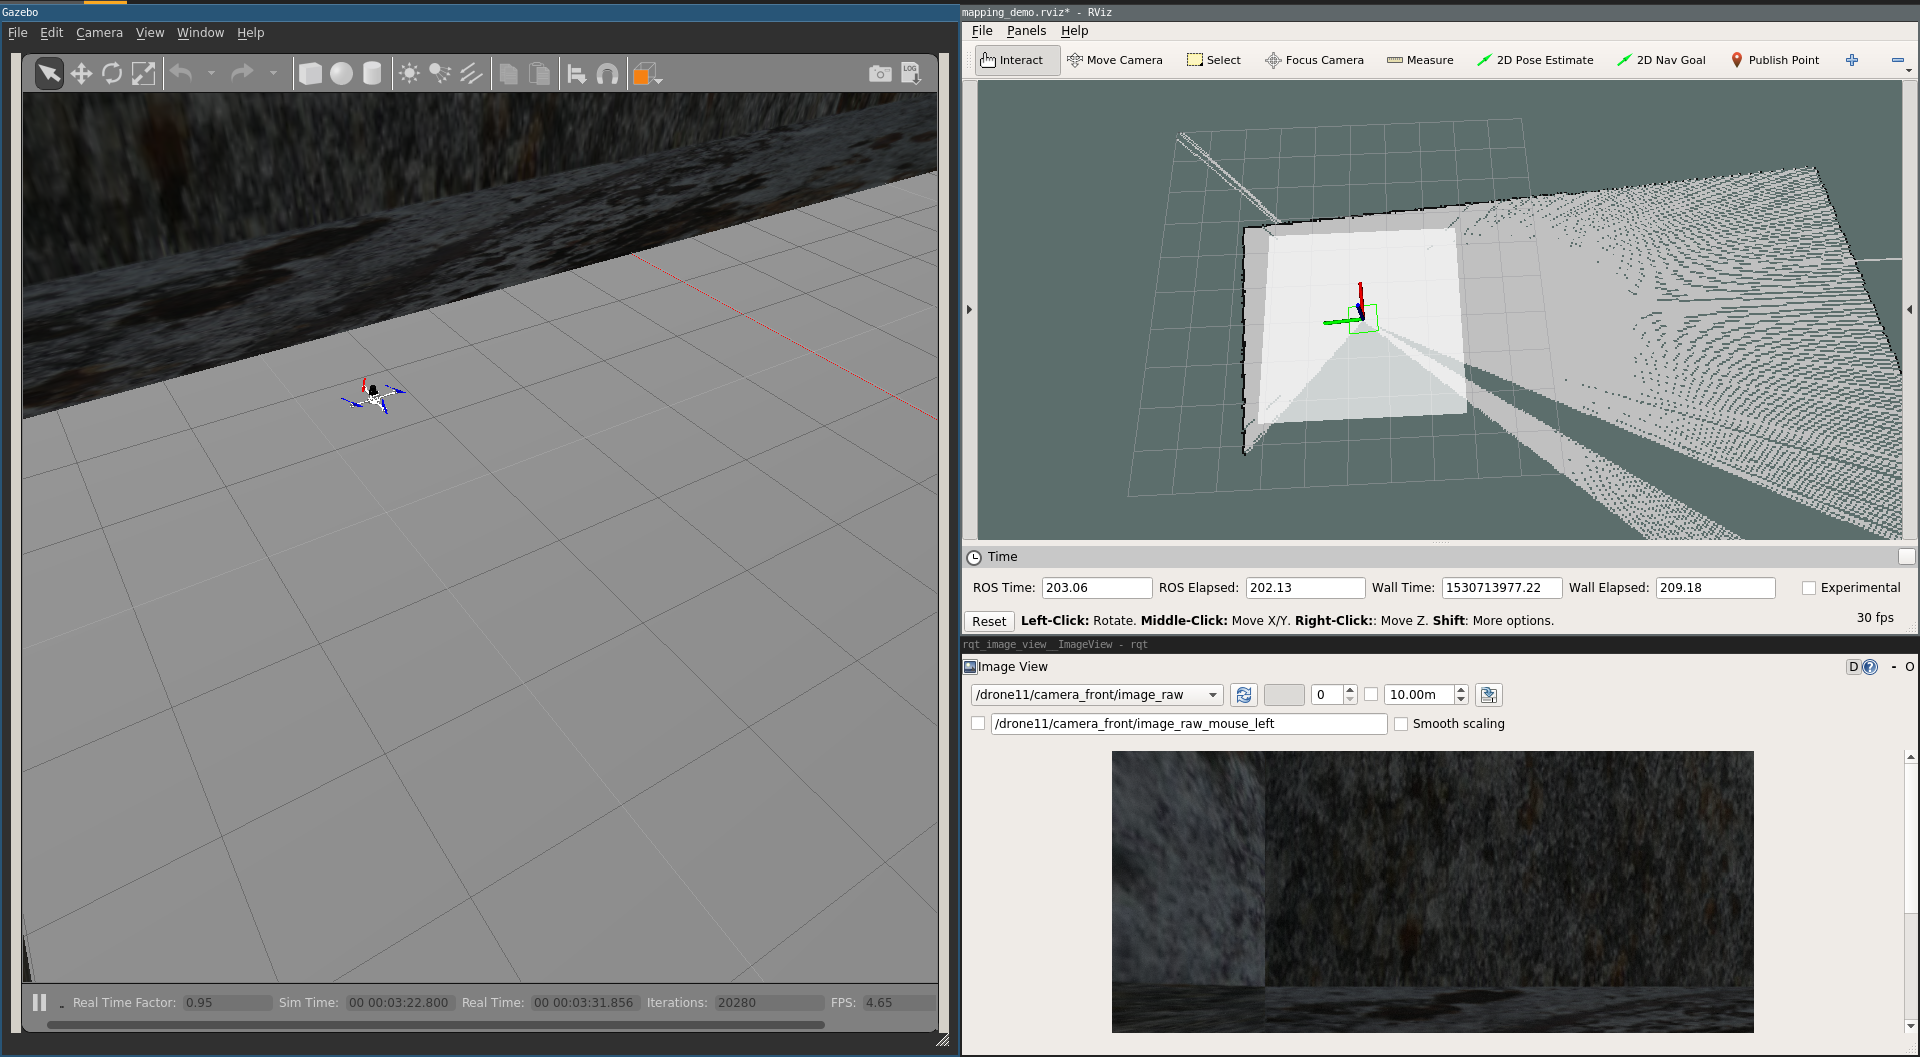
\includegraphics[width=0.9\textwidth,height=0.5\textheight,keepaspectratio]{./Figures/FullSim.png}
      \caption{Gazebo and Rviz. Simulation visualization during the execution of the mission. Left: Gazebo World, top-right: Rviz lidar measures, bottom-right: Hummingbird front camera}
      \label{ch_5:fig:full_sim}
    \end{figure}

  \subsection{Real Flight} \label{ch_5:subsect:exp_real_flight}

    For the real flight tests we used the sports centre in the School of Industrial Engineers, which is a closed space that can serve for our purposes, it's dimensions are listed in table \ref{ch_5:table:sports_dims}

    \begin{table}[!h]
      \centering
      \begin{tabular}{lr} \toprule
        \multicolumn{2}{c}{\textit{Sports Centre Dimensions}}        \\ \midrule
        Width $\times$ Depth $\times$ Height & $10 \times 25 \times 14$ \\ \bottomrule
        \hline
      \end{tabular}
      \caption{Dimensions of the sports centre used for real flight tests. Shool of Industrial Engineers}
      \label{ch_5:table:sports_dims}
    \end{table}

    The chosen drone ships a \href{https://www.dji.com/es/manifold}{DJI Manifold} micro computer for onboard computation. Its technical details are contained in table \ref{ch_5:table:manifold_specs}

    \begin{table}[!h]
      \centering
      \begin{tabular}{lr} \toprule
        \multicolumn{1}{c}{\textit{component}} & \multicolumn{1}{c}{\textit{value}}   \\ \midrule
        Ram           & DDR 3 2 GB     \\
        Processor     & 2.5 Ghz 4 cores \\
        GPU           & NVIDIA Kepler GeForce \\ \bottomrule
        \hline
      \end{tabular}
      \caption{Onboard computer specification}
      \label{ch_5:table:manifold_specs}
    \end{table}

    Onboard computation is the better option in this case because there is no \textit{auto pilot} (fallback driver controller, shipped in many drones to do automatic hover when no orders are received) and given the distances it can travel and the altitude, ensuring WiFi coverage is difficult. Hence, the most secure option is to load all the necessary software inside the onboard computer and send just a few orders from the ground control station. More specifically, launch the Aerostack and the python mission.

    The manifold computer is not very powerful so special attention must be put on perfomance, if computing power drains it can be catastrophic. To aid in this situation a human pilot was prepared to take control during all the tests, although at the end it was not necessary.

\section{Experimental Results} \label{ch_5:sect:results}

  This section will explain the results obtained

\section{Conclusions} \label{ch_5:sect:conclusions}

\begin{comment}
  \begin{itemize}
    \item Comment bullet
  \end{itemize}
\end{comment}
